\documentclass{extbook}[14pt]
\usepackage{multicol, enumerate, enumitem, hyperref, color, soul, setspace, parskip, fancyhdr, amssymb, amsthm, amsmath, bbm, latexsym, units, mathtools}
\everymath{\displaystyle}
\usepackage[headsep=0.5cm,headheight=0cm, left=1 in,right= 1 in,top= 1 in,bottom= 1 in]{geometry}
\usepackage{dashrule}  % Package to use the command below to create lines between items
\newcommand{\litem}[1]{\item #1

\rule{\textwidth}{0.4pt}}
\pagestyle{fancy}
\lhead{}
\chead{Answer Key for Progress Quiz 9 Version A}
\rhead{}
\lfoot{8590-6105}
\cfoot{}
\rfoot{Fall 2020}
\begin{document}
\textbf{This key should allow you to understand why you choose the option you did (beyond just getting a question right or wrong). \href{https://xronos.clas.ufl.edu/mac1105spring2020/courseDescriptionAndMisc/Exams/LearningFromResults}{More instructions on how to use this key can be found here}.}

\textbf{If you have a suggestion to make the keys better, \href{https://forms.gle/CZkbZmPbC9XALEE88}{please fill out the short survey here}.}

\textit{Note: This key is auto-generated and may contain issues and/or errors. The keys are reviewed after each exam to ensure grading is done accurately. If there are issues (like duplicate options), they are noted in the offline gradebook. The keys are a work-in-progress to give students as many resources to improve as possible.}

\rule{\textwidth}{0.4pt}

\begin{enumerate}\litem{
Describe the end behavior of the polynomial below.
\[ f(x) = -6(x - 7)^{3}(x + 7)^{8}(x + 2)^{3}(x - 2)^{3} \]

The solution is the graph below, which is option A.
\begin{center}
    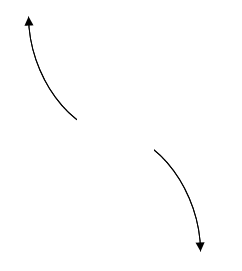
\includegraphics[width=0.3\textwidth]{../Figures/polyEndBehaviorAA.png}
\end{center}\begin{enumerate}[label=\Alph*.]
\begin{multicols}{2}
\item 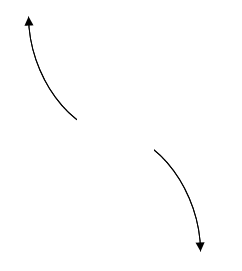
\includegraphics[width = 0.3\textwidth]{../Figures/polyEndBehaviorAA.png}
\item 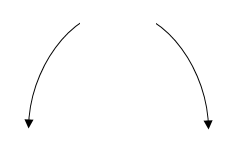
\includegraphics[width = 0.3\textwidth]{../Figures/polyEndBehaviorBA.png}
\item 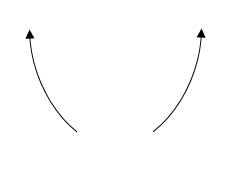
\includegraphics[width = 0.3\textwidth]{../Figures/polyEndBehaviorCA.png}
\item 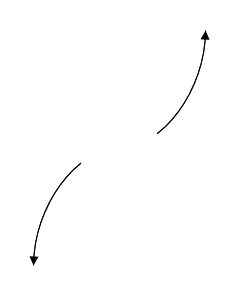
\includegraphics[width = 0.3\textwidth]{../Figures/polyEndBehaviorDA.png}
\end{multicols}\item None of the above.\end{enumerate}
\textbf{General Comment:} Remember that end behavior is determined by the leading coefficient AND whether the \textbf{sum} of the multiplicities is positive or negative.
}
\litem{
Which of the following equations \textit{could} be of the graph presented below?

\begin{center}
    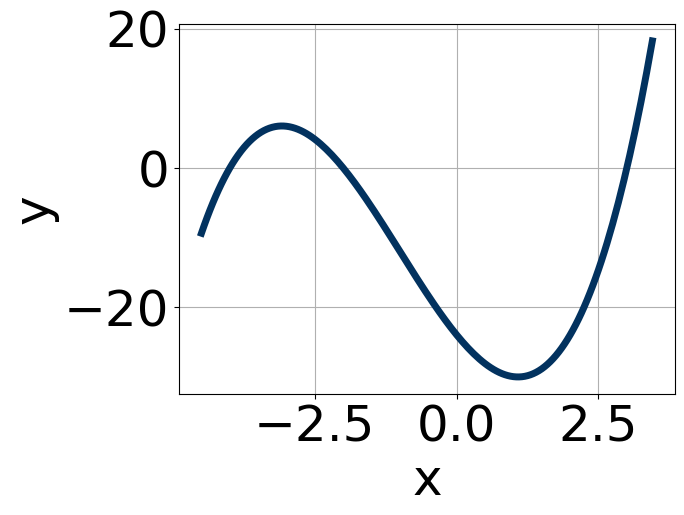
\includegraphics[width=0.5\textwidth]{../Figures/polyGraphToFunctionCopyA.png}
\end{center}




The solution is \( -20x^{4} (x - 1)^{6} (x + 2)^{7} \), which is option E.\begin{enumerate}[label=\Alph*.]
\item \( 8x^{4} (x - 1)^{4} (x + 2)^{11} \)

This corresponds to the leading coefficient being the opposite value than it should be.
\item \( -15x^{4} (x - 1)^{11} (x + 2)^{10} \)

The factor $(x - 1)$ should have an even power and the factor $(x + 2)$ should have an odd power.
\item \( -3x^{10} (x - 1)^{9} (x + 2)^{11} \)

The factor $(x - 1)$ should have an even power.
\item \( 16x^{8} (x - 1)^{8} (x + 2)^{4} \)

The factor $(x + 2)$ should have an odd power and the leading coefficient should be the opposite sign.
\item \( -20x^{4} (x - 1)^{6} (x + 2)^{7} \)

* This is the correct option.
\end{enumerate}

\textbf{General Comment:} General Comments: Draw the x-axis to determine which zeros are touching (and so have even multiplicity) or cross (and have odd multiplicity).
}
\litem{
Construct the lowest-degree polynomial given the zeros below. Then, choose the intervals that contain the coefficients of the polynomial in the form $ax^3+bx^2+cx+d$.
\[ \frac{-2}{3}, \frac{4}{5}, \text{ and } \frac{-5}{4} \]

The solution is \( 60x^{3} +67 x^{2} -42 x -40 \), which is option C.\begin{enumerate}[label=\Alph*.]
\item \( a \in [51, 65], b \in [-78, -65], c \in [-43, -39], \text{ and } d \in [40, 46] \)

$60x^{3} -67 x^{2} -42 x + 40$, which corresponds to multiplying out $(3x -2)(5x + 4)(4x -5)$.
\item \( a \in [51, 65], b \in [64, 74], c \in [-43, -39], \text{ and } d \in [40, 46] \)

$60x^{3} +67 x^{2} -42 x + 40$, which corresponds to multiplying everything correctly except the constant term.
\item \( a \in [51, 65], b \in [64, 74], c \in [-43, -39], \text{ and } d \in [-41, -38] \)

* $60x^{3} +67 x^{2} -42 x -40$, which is the correct option.
\item \( a \in [51, 65], b \in [82, 84], c \in [-26, -18], \text{ and } d \in [-41, -38] \)

$60x^{3} +83 x^{2} -22 x -40$, which corresponds to multiplying out $(3x -2)(5x + 4)(4x + 5)$.
\item \( a \in [51, 65], b \in [-13, -11], c \in [-83, -76], \text{ and } d \in [40, 46] \)

$60x^{3} -13 x^{2} -78 x + 40$, which corresponds to multiplying out $(3x -2)(5x -4)(4x + 5)$.
\end{enumerate}

\textbf{General Comment:} To construct the lowest-degree polynomial, you want to multiply out $(3x + 2)(5x -4)(4x + 5)$
}
\litem{
Construct the lowest-degree polynomial given the zeros below. Then, choose the intervals that contain the coefficients of the polynomial in the form $ax^3+bx^2+cx+d$.
\[ 5, \frac{7}{4}, \text{ and } \frac{1}{4} \]

The solution is \( 16x^{3} -112 x^{2} +167 x -35 \), which is option A.\begin{enumerate}[label=\Alph*.]
\item \( a \in [12, 26], b \in [-113, -109], c \in [157, 171], \text{ and } d \in [-45, -34] \)

* $16x^{3} -112 x^{2} +167 x -35$, which is the correct option.
\item \( a \in [12, 26], b \in [102, 105], c \in [113, 118], \text{ and } d \in [-45, -34] \)

$16x^{3} +104 x^{2} +113 x -35$, which corresponds to multiplying out $(x + 5)(4x + 7)(4x -1)$.
\item \( a \in [12, 26], b \in [48, 52], c \in [-153, -150], \text{ and } d \in [34, 42] \)

$16x^{3} +48 x^{2} -153 x + 35$, which corresponds to multiplying out $(x + 5)(4x -7)(4x -1)$.
\item \( a \in [12, 26], b \in [112, 116], c \in [157, 171], \text{ and } d \in [34, 42] \)

$16x^{3} +112 x^{2} +167 x + 35$, which corresponds to multiplying out $(x + 5)(4x + 7)(4x + 1)$.
\item \( a \in [12, 26], b \in [-113, -109], c \in [157, 171], \text{ and } d \in [34, 42] \)

$16x^{3} -112 x^{2} +167 x + 35$, which corresponds to multiplying everything correctly except the constant term.
\end{enumerate}

\textbf{General Comment:} To construct the lowest-degree polynomial, you want to multiply out $(x -5)(4x -7)(4x -1)$
}
\litem{
Construct the lowest-degree polynomial given the zeros below. Then, choose the intervals that contain the coefficients of the polynomial in the form $x^3+bx^2+cx+d$.
\[ 4 - 5 i \text{ and } -2 \]

The solution is \( x^{3} -6 x^{2} +25 x + 82 \), which is option D.\begin{enumerate}[label=\Alph*.]
\item \( b \in [0.3, 3.1], c \in [5, 10], \text{ and } d \in [8, 12] \)

$x^{3} + x^{2} +7 x + 10$, which corresponds to multiplying out $(x + 5)(x + 2)$.
\item \( b \in [2.1, 8.9], c \in [15, 28], \text{ and } d \in [-89, -71] \)

$x^{3} +6 x^{2} +25 x -82$, which corresponds to multiplying out $(x-(4 - 5 i))(x-(4 + 5 i))(x -2)$.
\item \( b \in [0.3, 3.1], c \in [-3, -1], \text{ and } d \in [-8, -3] \)

$x^{3} + x^{2} -2 x -8$, which corresponds to multiplying out $(x -4)(x + 2)$.
\item \( b \in [-7.3, -5.9], c \in [15, 28], \text{ and } d \in [82, 85] \)

* $x^{3} -6 x^{2} +25 x + 82$, which is the correct option.
\item \( \text{None of the above.} \)

This corresponds to making an unanticipated error or not understanding how to use nonreal complex numbers to create the lowest-degree polynomial. If you chose this and are not sure what you did wrong, please contact the coordinator for help.
\end{enumerate}

\textbf{General Comment:} Remember that the conjugate of $a+bi$ is $a-bi$. Since these zeros always come in pairs, we need to multiply out $(x-(4 - 5 i))(x-(4 + 5 i))(x-(-2))$.
}
\litem{
Construct the lowest-degree polynomial given the zeros below. Then, choose the intervals that contain the coefficients of the polynomial in the form $x^3+bx^2+cx+d$.
\[ -3 - 5 i \text{ and } 3 \]

The solution is \( x^{3} +3 x^{2} +16 x -102 \), which is option D.\begin{enumerate}[label=\Alph*.]
\item \( b \in [-0.42, 1.63], c \in [-3.2, 1], \text{ and } d \in [-14, -6] \)

$x^{3} + x^{2} -9$, which corresponds to multiplying out $(x + 3)(x -3)$.
\item \( b \in [-4.7, -1.52], c \in [14.7, 18.4], \text{ and } d \in [102, 106] \)

$x^{3} -3 x^{2} +16 x + 102$, which corresponds to multiplying out $(x-(-3 - 5 i))(x-(-3 + 5 i))(x + 3)$.
\item \( b \in [-0.42, 1.63], c \in [1.8, 4.8], \text{ and } d \in [-17, -13] \)

$x^{3} + x^{2} +2 x -15$, which corresponds to multiplying out $(x + 5)(x -3)$.
\item \( b \in [2.39, 3.09], c \in [14.7, 18.4], \text{ and } d \in [-107, -92] \)

* $x^{3} +3 x^{2} +16 x -102$, which is the correct option.
\item \( \text{None of the above.} \)

This corresponds to making an unanticipated error or not understanding how to use nonreal complex numbers to create the lowest-degree polynomial. If you chose this and are not sure what you did wrong, please contact the coordinator for help.
\end{enumerate}

\textbf{General Comment:} Remember that the conjugate of $a+bi$ is $a-bi$. Since these zeros always come in pairs, we need to multiply out $(x-(-3 - 5 i))(x-(-3 + 5 i))(x-(3))$.
}
\litem{
Describe the zero behavior of the zero $x = -2$ of the polynomial below.
\[ f(x) = -9(x - 5)^{6}(x + 5)^{5}(x - 2)^{11}(x + 2)^{6} \]

The solution is the graph below, which is option C.
\begin{center}
    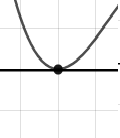
\includegraphics[width=0.3\textwidth]{../Figures/polyZeroBehaviorCopyCA.png}
\end{center}\begin{enumerate}[label=\Alph*.]
\begin{multicols}{2}
\item 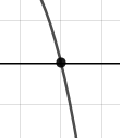
\includegraphics[width = 0.3\textwidth]{../Figures/polyZeroBehaviorCopyAA.png}
\item 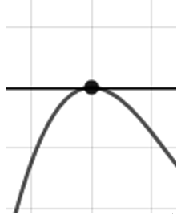
\includegraphics[width = 0.3\textwidth]{../Figures/polyZeroBehaviorCopyBA.png}
\item 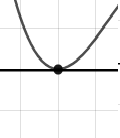
\includegraphics[width = 0.3\textwidth]{../Figures/polyZeroBehaviorCopyCA.png}
\item 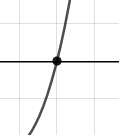
\includegraphics[width = 0.3\textwidth]{../Figures/polyZeroBehaviorCopyDA.png}
\end{multicols}\item None of the above.\end{enumerate}
\textbf{General Comment:} You will need to sketch the entire graph, then zoom in on the zero the question asks about.
}
\litem{
Describe the end behavior of the polynomial below.
\[ f(x) = -5(x + 8)^{2}(x - 8)^{5}(x + 7)^{3}(x - 7)^{3} \]

The solution is the graph below, which is option A.
\begin{center}
    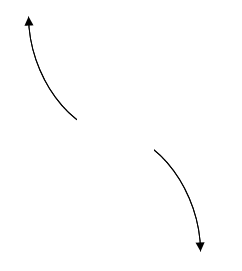
\includegraphics[width=0.3\textwidth]{../Figures/polyEndBehaviorCopyAA.png}
\end{center}\begin{enumerate}[label=\Alph*.]
\begin{multicols}{2}
\item 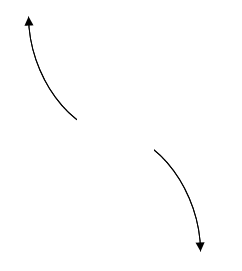
\includegraphics[width = 0.3\textwidth]{../Figures/polyEndBehaviorCopyAA.png}
\item 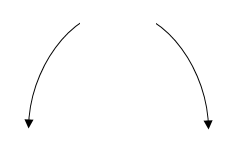
\includegraphics[width = 0.3\textwidth]{../Figures/polyEndBehaviorCopyBA.png}
\item 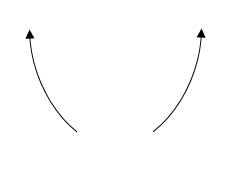
\includegraphics[width = 0.3\textwidth]{../Figures/polyEndBehaviorCopyCA.png}
\item 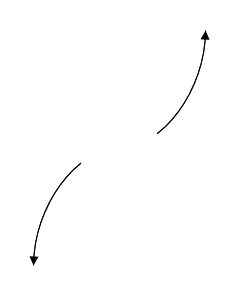
\includegraphics[width = 0.3\textwidth]{../Figures/polyEndBehaviorCopyDA.png}
\end{multicols}\item None of the above.\end{enumerate}
\textbf{General Comment:} Remember that end behavior is determined by the leading coefficient AND whether the \textbf{sum} of the multiplicities is positive or negative.
}
\litem{
Which of the following equations \textit{could} be of the graph presented below?

\begin{center}
    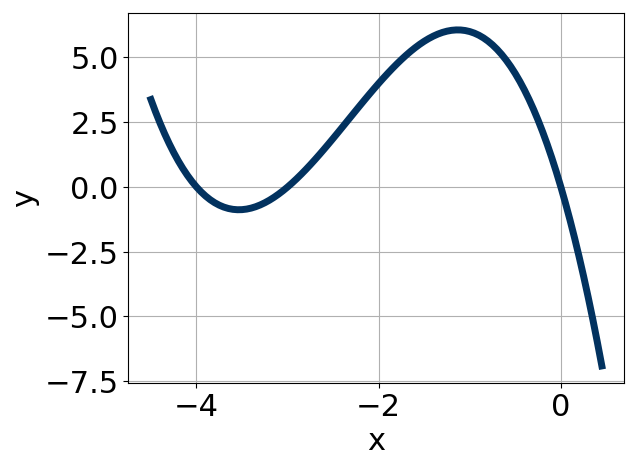
\includegraphics[width=0.5\textwidth]{../Figures/polyGraphToFunctionA.png}
\end{center}




The solution is \( 20(x + 4)^{11} (x + 1)^{7} (x + 2)^{11} \), which is option C.\begin{enumerate}[label=\Alph*.]
\item \( -4(x + 4)^{9} (x + 1)^{9} (x + 2)^{5} \)

This corresponds to the leading coefficient being the opposite value than it should be.
\item \( -2(x + 4)^{4} (x + 1)^{5} (x + 2)^{11} \)

The factor $(x + 4)$ should have an odd power and the leading coefficient should be the opposite sign.
\item \( 20(x + 4)^{11} (x + 1)^{7} (x + 2)^{11} \)

* This is the correct option.
\item \( 10(x + 4)^{4} (x + 1)^{9} (x + 2)^{11} \)

The factor $-4$ should have been an odd power.
\item \( 12(x + 4)^{10} (x + 1)^{8} (x + 2)^{7} \)

The factors $-4$ and $-1$ have have been odd power.
\end{enumerate}

\textbf{General Comment:} General Comments: Draw the x-axis to determine which zeros are touching (and so have even multiplicity) or cross (and have odd multiplicity).
}
\litem{
Describe the zero behavior of the zero $x = 2$ of the polynomial below.
\[ f(x) = -7(x + 2)^{2}(x - 2)^{7}(x + 7)^{3}(x - 7)^{4} \]

The solution is the graph below, which is option A.
\begin{center}
    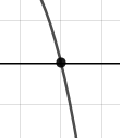
\includegraphics[width=0.3\textwidth]{../Figures/polyZeroBehaviorAA.png}
\end{center}\begin{enumerate}[label=\Alph*.]
\begin{multicols}{2}
\item 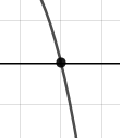
\includegraphics[width = 0.3\textwidth]{../Figures/polyZeroBehaviorAA.png}
\item 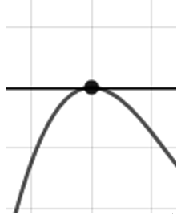
\includegraphics[width = 0.3\textwidth]{../Figures/polyZeroBehaviorBA.png}
\item 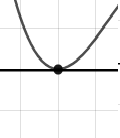
\includegraphics[width = 0.3\textwidth]{../Figures/polyZeroBehaviorCA.png}
\item 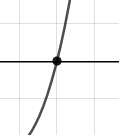
\includegraphics[width = 0.3\textwidth]{../Figures/polyZeroBehaviorDA.png}
\end{multicols}\item None of the above.\end{enumerate}
\textbf{General Comment:} You will need to sketch the entire graph, then zoom in on the zero the question asks about.
}
\end{enumerate}

\end{document}